\section{Results: normal-tissue expression background of the panel (GTEx v8)}
\label{sec:gtex}
The gnomAD audit (Sec.~\ref{sec:gnomad}) validates the panel at the DNA level;
here we test the complementary question at the RNA level: does any panel gene
carry expression-level pancreatic specificity that an assay could exploit, and
what normal background does the blood compartment contribute? We fetched
per-sample GTEx v8 TPM vectors for the four panel genes plus four controls
(housekeeping GAPDH, ACTB; pancreas-specific PRSS1, INS) from the GTEx Portal
API -- 54 tissues, 17,382 samples per gene, 432 tissue$\times$gene median
records (\texttt{results/gtex\_panel\_tissue\_medians.csv}) -- and computed
median TPM per tissue, the $\tau$ tissue-specificity index
$\tau=\frac{1}{n-1}\sum_i\left(1-x_i/x_{\max}\right)$, and the pancreas rank
among tissues. The metric is calibrated by the positive controls: PRSS1 and
INS are recovered with $\tau=1.000$, pancreas rank 1/54 and pancreas-to-blood
ratios of $3.3\times10^{5}$ and $\ge2.3\times10^{3}$.

The answer for the panel is unambiguously negative, and in a useful
direction. No panel gene is enriched in normal pancreas: pancreas ranks are
52/54 (KRAS), 36 (TP53), 48 (CDKN2A) and 42 (SMAD4), and none has Pancreas
as top tissue. Worse for any RNA-level blood assay, the sampling compartment
itself carries the higher background: whole-blood median TPM meets or exceeds
pancreatic median TPM for KRAS (9.09 vs 5.03) and TP53 (7.70 vs 7.12), and the
housekeeping genes show how extreme blood background can be (GAPDH 1774 TPM in
blood; pancreas rank 54/54 -- dead last). CDKN2A is near-silent in both normal
pancreas (0.216 TPM) and blood (0.285 TPM), consistent with p16 induction on
stress rather than basal expression; its high $\tau$ (0.93) reflects pituitary
expression, not pancreas. Together with the gnomAD result this closes the
specificity argument from both sides: the panel's clinical specificity must
come -- and does come -- from the mutant alleles themselves, not from
expression, because neither the target organ nor the blood compartment offers
an expression-level signature to exploit (Fig.~\ref{fig:gtex}).
\begin{figure}[h]\centering
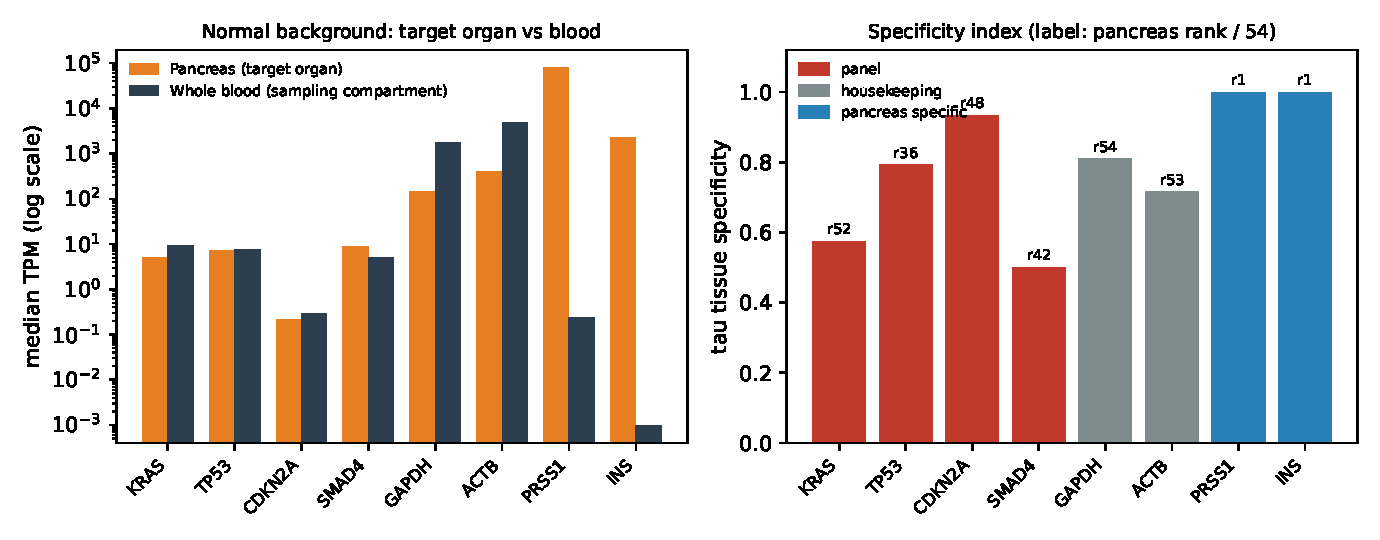
\includegraphics[width=0.98\linewidth]{figs/fig_gtex_background.pdf}
\caption{Left: normal-tissue median TPM in pancreas (target organ) versus
whole blood (the liquid-biopsy sampling compartment) for the four panel genes
and four controls (log scale). Right: $\tau$ tissue-specificity index per
gene, annotated with the pancreas expression rank among 54 tissues; only the
pancreas-specific controls PRSS1/INS achieve high $\tau$ via pancreas.}
\label{fig:gtex}\end{figure}
